% !TEX root = ../thesis.tex
\makeatletter
\def\input@path{{../}}
\makeatother
\documentclass[../thesis.tex]{subfiles}
\begin{document}

\selectlanguage{english}
	
\section{Numerical Experiment}
We performed a numerical simulation of the fixed-state free-final-time control for double integrator model, as well as the kinodynamic-RRT* in dynamic environment to verify this algorithm. This numerical simulation were executed on Laptop PC with Intel Core i3 2.0 GHz processor, 4 GB memory and Ubuntu 16.04 Operating System. First, we performed the numerical simulation of the fixed-state free-final-time control by evaluating the resulting trajectory given various input weights. Secondly, we performed a numerical simulation for the kinodynamic-RRT* with double integrator model and in dynamic environment and evaluated the resulting motion plan. Thirdly, we performed a numerical simulation of minimum-time trajectory generator for the robot's orientation.

\subsection{Fixed-State Free-Final-Time Control for Double Integrator Model}
In this section, we evaluated our experiment on the fixed-state free-final-time control for the double integrator model. We compared the trajectories of the model across different value of input weight, $r$, from similar value initial and final state. We also compared the maximum control input among the trajectories.

\begin{table}[]
\caption{Arrival Time and Maximum Control Input for Several Input Weight}
\label{trajectories_table}
\centering
\begin{tabular}{|l|l|l|}
\hline
$r$ & arrival time (s) & maximum $\| u \|$ \\ \hline
$1.5$ & $6.9187936337$ & $1.2253000912634624$ \\ \hline
$1.0$ & $6.05276367644$ & $1.467295152420136$ \\ \hline
$0.5$ & $4.84707681233$ & $1.997746119057331$ \\ \hline
\end{tabular}
\end{table}
Table \ref{trajectories_table} shows the arrival time and the maximum control input for each input weights, where $\|u\| = \sqrt{u_x^2+u_y^2}$. It could be noted that the input weight affects the arrival time and the control input given to the system. With $r=1.5$, the controller penalized more acceleration and arrive in $6.9187936337$ s given $x_i$ and $x_f$ value with the lowest maximum control input among others, $1.2253000912634624$. With lower $r=1.0$, the maximum control input becomes larger, $\|u\|=1.467295152420136$ and arrives faster at $6.05276367644$ s. Finally with more lower input weight, $r=0.5$, the controller exerted more larger input, with $\|u\|=1.997746119057331$ but also the fastest arrive to the final state in $4.84707681233$ s among other input weight configuration.

It has shown that the input weighting parameter, $r$, affects the arrival time and the control effort. The larger input weight results on longer arrival time but lower control effort while smaller input weight results results on faster arrival time with larger control effort. We used this input weighting parameter as \emph{soft constraint} of the trajectory.

\subsection{Kinodynamic-RRT* for Double Integrator Model}
In this section, we evaluated our numerical experiment on motion planning for double integrator model using the kinodynamic-RRT* algorithm. The implemented kinodynamic-RRT* for double integrator model is written using C++ programming language within Robot Operating System (ROS) framework. The grown tree of the kinodynamic-RRT* is also visualized with RViz by publishing the tree via ROS message. In this numerical experiment, we consider safety,  cost and computation times of the solution trajectory. Furthermore, we also consider the effect of direct sampling to the solution cost and computation time of the kinodynamic-RRT*. 

\begin{table}[H]
\caption{Numerical Experiment Parameter}
\label{param_table}
\centering
\begin{tabular}{|l|l|}
\hline
parameter                 & value \\ \hline
input weight, $r$          & $1.0$   \\ \hline
initial state, $q_{start}$ & $[-3.0, -0.5, 1.3, -0.9]^T$      \\ \hline
goal state, $q_{goal}$     & $[4.97, 6.78, 0.0, 0.0]^T$      \\ \hline
\multirow{9}{*}{Obstacles} & $[8.83019,6.98859,-1.17926,-0.451501]^T$ \\ \cline{2-2} 
                           & $[-1.52327,0.0548198,-1.27471,0.2655]$ \\ \cline{2-2} 
                           & $[-3.92824,0.335711,1.1615,-0.726765]^T$ \\ \cline{2-2} 
                           & $[5.82367,0.359309,1.10046,1.38117]^T$ \\ \cline{2-2} 
                           & $[6.5626,-0.423526,1.39883,0.820934]^T$ \\ \cline{2-2} 
                           & $[-1.75533,0.41505,-1.15699,0.587055]^T$ \\ \cline{2-2} 
                           & $[-1.52264,-5.707,-1.41173,-0.421272]^T$ \\ \cline{2-2} 
                           & $[-0.931017,-4.5069,-1.3309,-1.33343]^T$ \\ \cline{2-2} 
                           & $[-7.65285,5.12917,-0.479974,1.31268]^T$ \\ \hline
\end{tabular}
\end{table}

For this numerical experiment, we use the configuration and parameter as shown in table \ref{param_table}. In the table the input weight are the weighting value for the optimal controller.The initial and goal state, $q_{start}$ and $q_{goal}$, are the double integrator states represented as vectors consist of position and velocity, $[x,y,\dot{x},\dot{y}]^T$, in $m$ and $m/s$ for position and velocity respectively. In this experiment, we used $9$ moving obstacles. The obstacles are modeled as moving circle with constant speed.

\subsubsection{Solution Cost}
Figure \ref{plot_compare_cost} shows the data of solution costs from $100$ times of experiment with and without direct sampling. Figure \ref{plot_compare_cost:no} shows the solution cost without directly sampling the goal state and figure \ref{plot_compare_cost:0.1} shows the distribution of the solution cost with direct sampling to the goal with $0.1$ probability. 

Without direct sampling to goal state, the median of solution costs becomes smaller as the number of node increases, while with direct sampling to the goal state, the median of the costs is already on the lower range of solution costs even with smaller number of nodes and further increase the number of nodes does not reduces the median of solution costs. On both cases, however, increasing the number of nodes tends to reduce the range of maximum costs.

It is shown that by directly sampling the goal state, the solution costs are more concentrated on the lowest possible cost. This implies that by directly sampling the goal state, it produces more consistent and lower solution cost. 

\begin{figure}[H]
	\centering
	\begin{subfigure}{1\textwidth}
		\centering
		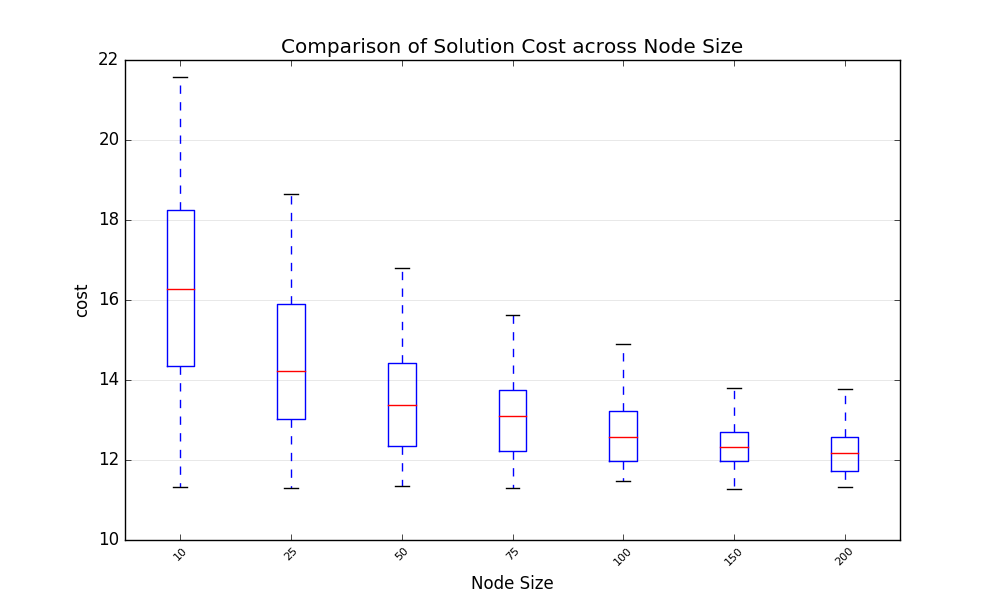
\includegraphics[width=14cm]{boxplot_cost_no}
		\caption{Solution Cost without Direct Sampling}
		\label{plot_compare_cost:no}
	\end{subfigure}
	\begin{subfigure}{1\textwidth}
		\centering
		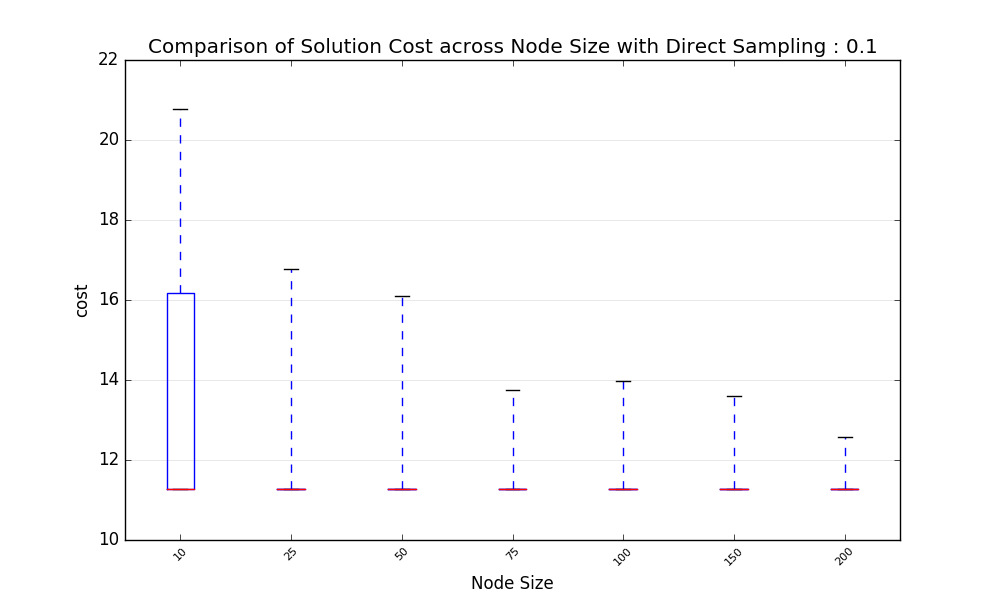
\includegraphics[width=14cm]{boxplot_cost_01}
		\caption{Solution Cost without Direct Sampling with $p=0.1$}
		\label{plot_compare_cost:0.1}
	\end{subfigure}
	\caption{Comparison of Solution Cost with and without Direct Sampling}
	\label{plot_compare_cost}
\end{figure}

\subsection{Minimum-Time Trajectory for Rotational Motion}
In this section, we evaluated our numerical experiment on minimum-time trajectory for rotational motion of omnidirectional robot. We performed our numerical experiment on two cases using different initial state. Table \ref{angular_exp_table} shows the experiments settings.

\section{Dynamic Simulation Experiment}

In this section, we discuss the result of our dynamic simulation experiment in physical simulator environment. In this experiment, we ran the designed motion planning system in robot soccer environment with dynamic obstacles. In such scenario, the exact motion of the obstacles at any given time is not available, but only the states, e.g. position and velocity, of the obstacles are known. First we discuss our approach to the problem where the exact motion of obstacles are not available. Second, we discuss the simulation system of this experiment. And finally we discuss the results of the experiment. Our implementation of the system is available at \url{https://bitbucket.org/alifahrri/robosoccer_motion_planning_ws/}.

\subsection{Simulation System}
Figure \ref{rosgraph} shows the software component of our experiment. In the figure, a rectangle block represents ROS Topic and an ellipse represents an executable ROS Node. The arrows show the interaction of nodes via topics, an incoming arrows represent subscribed topics and an outcoming arrows represent published topics. The figure was produced using standard ros package to visualize computational graph, $\vars{rqt\_graph}$.

The executable ROS Node in this experiments consists of the following elements :

\begin{itemize}
\item{$\vars{/gazebo}$} this ROS Node is responsible for providing physics simulation for the experiment. This node is provided by standard ROS distribution as standard package $\vars{gazebo\_ros}$. In this experiment, this node published the topics : $\vars{/robot/omnivision/OmniVisionInfo}$, where $\vars{robot}$ is the robot's name, that provides the information of the robot states (pose and twist). Those topics are provided by the robot soccer simulation system from \cite{yao2015simulation}. The simulation system could also controls individual robot's movement by subscribing the topics $\vars{/robot/nubotcontrol/velcmd}$, where \vars{robot} is the robot's name, that will tell \vars{/gazebo} node to move the robot's physical model.
\item{$\vars{/robosoccer\_motion\_planning}$} 
\justify{
is our ROS implementation of our motion planning system described in chapter 3. This node was written in C++ programming language and is responsible for computing the collision-free trajectories and publish it as ROS topics. The node receive the information necessary for the motion planning system, that is the robot's state and environment (obstacles), from the \vars{/gazebo} node by subscribing to topics for \vars{nubot1} and \vars{rival1}. Furthermore, we can send the goal target by publishing $\vars{/move\_base\_simple/goal}$ which is also subscribed by the node. In this experiment, we sent $\vars{/move\_base\_simple/goal}$ messages via \vars{/rviz} node and $\vars{/robosoccer\_teleop\_node}$. The resulting trajectory plan consists of planned time-parametrized position and velocity :
}
\begin{itemize}[label=$\star$]
\item{$\vars{/robosoccer\_trajectory\_pos}$} 
\item{$\vars{/robosoccer\_trajectory\_vel}$}
\end{itemize}
both of the topic above has message type of $\vars{nav\_msgs/PoseStamped}$, which is included in standard ROS distribution. The message consists of array of time stamped pose. The time is synchronized over other messages and nodes via the \vars{/clock} topic. This node also publish $\vars{/rrt\_msgs}$ which provides visualization data of the grown tree, obstacles, and the solution trajectory that are to be visualized in \vars{/rviz} node.
\item{$\vars{/robosoccer\_trajectory\_tracking}$} node is our implementation of the trajectory tracking discussed in chapter 3. The node was written in Python programming language. This node is responsible for controlling the robot to following the solution trajectory provided by the motion planning system. The computed velocity command of the robot is sent to the \vars{/gazebo} node to move the robot's physical model.
\item{$\vars{/robosoccer\_teleop}$}node is our software implementation to move 'dummy' obstacles to simulate the dynamic environment written in Python programming language. To move the 'dummy' obstacles, we applied proportional derivative (PD) position control to follows a set of waypoint of each robot. The waypoints is built via interactive GUI as depicted in figure \ref{robosoccer_teleop}. The gui was built using PyQt library \cite{computing2013pyqt}. After the control command is computed, the node is then publish the control command for the 'dummy' obstacles to \vars{/gazebo} node. Besides, we also use this node to publish waypoint of goals to the motion planning system via \vars{/move\_base\_simple/goal} topic. To achieve this, we subscribe to the robot's state topic and checks if the robot is already arrive at specified waypoint then the next goal is published. In figure \ref{robosoccer_teleop}, each big circle represents robot's position while smaller circle represents waypoints for each robots with active target positions are shown with green color.
\item{$\vars{/rviz}$} node is used in this experiment to visualize the explored tree, the solution trajectory, the current robot position, and the dynamic obstacles. This node is part of standard ROS distribution.
\end{itemize}

\end{document}